\vspace{2cm}
\section{Auswertung} 

\underline{\textbf{Statische Methode}}


\begin{figure}[H]
    \centering
    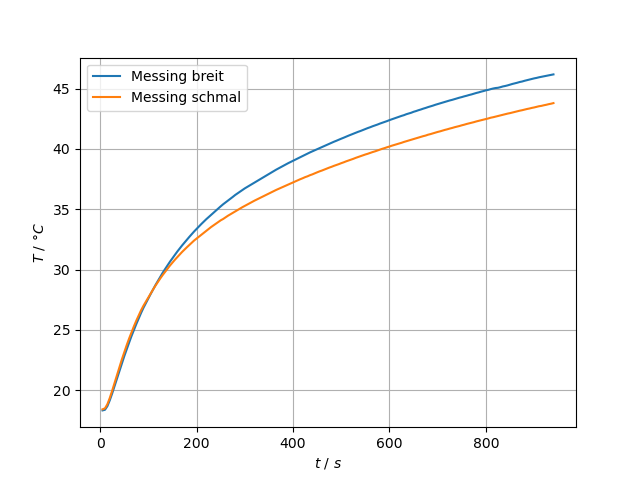
\includegraphics[height=80mm]{bilder/TemprVerlStT1T4.png}
    \caption{ Die Abbildung der zeitlichen Temperaturverläufe, mit der statischen Methode, von dem breiten Messingstab ($T_{1}$) und dem schmalen Messingstab ($T_{4}$). \label{Abbildung3} }
\end{figure}

\begin{flushleft}
    Die Graphen, sowohl $T_{1}$ und $ T_{4} $, steigen exponentiell. 
    Ab einer Zeit von ungefähr 125\,\unit{\second} trennen sich die Graphen,dabei steigt der breite Messingstab ($T_{1}$) stärker an als der schmale Messingstab ($T_{4}$),
    doch die Verlaufskurven ähneln sich.
\end{flushleft}

\begin{figure}[H]
    \centering
    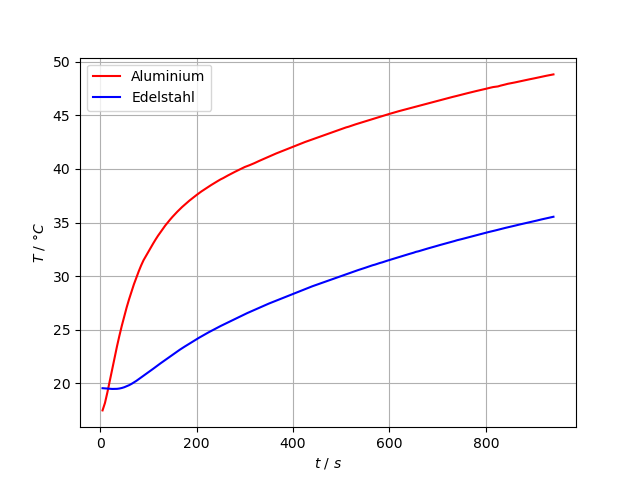
\includegraphics[height=80mm]{bilder/TemprVerlStT5T8.png}
    \caption{ Die Abbildung der zeitlichen Temperaturverläufe, mit der statischen Methode, von dem Aluminiumstab ($T_{5}$) und dem Edelstahlstab ($T_{8}$). \label{Abbildung4} }
\end{figure}


\begin{flushleft}
    Die Verläufe der Graphen verhalten sich in Abbildung \ref{Abbildung4} unterschiedlich, wobei die Temperatur des Aluminiumstabes ($T_{5}$) exponentiell ansteigt und nach längerer Zeit abflacht.
    Der Edelstahlstab ($T_{8}$) ist am Anfang abgeflacht und nimmt dann nach zunehmender Zeit wieder zu. Die Temperatur des Edelstahlstabes ist deutlich niedriger als die des Aluminiumstabes.
\end{flushleft}

\begin{align*}
    \intertext{Die Temperaturen, die nach 700\,\unit{\second} gemessen werden:} \\
    T_{1} = 317,15\,\unit{\kelvin} = 44\,\unit{\degreeCelsius}\\
    T_{4} = 314,65\,\unit{\kelvin} = 41,50\,\unit{\degreeCelsius}\\
    T_{5} = 319,53\,\unit{\kelvin} = 46,38\,\unit{\degreeCelsius}\\
    T_{8} = 306,65\,\unit{\kelvin} = 33,50\,\unit{\degreeCelsius}\\
\end{align*}

\begin{flushleft}
    Wie zu erkennen, hat das Thermoelement $T_{5}$ (Aluminiumstab) nach $700\,\unit{\second}$ die höchste Temperatur erreicht. 
    Daraus folgt, dass der Aluminiumstab die beste Wärmeleitung besitzt.
\end{flushleft}



\begin{flushleft}
    Um den Wärmestrom zu bestimmen,werden jeweils die Temperaturen der Differenz $ T_{2} - T_{1}$ und $ T_{7} - T_{8}$ zu fünf verschiedenen Zeiten bestimmt.
    Der Abstand der Thermo-Elemente beträgt $ \increment x_{\text{Edelstahl, Messing}} = (0,035 \pm 0,000)\,\unit{\meter} $.
    Die jeweiligen Werte von $\kappa$ werden aus den Vorbereitungsaufgaben entnommen und die Fläche A aus dem Versuchsblatt \cite{a1}. 
    Der Wärmestrom lässt sich durch die Formel \ref{1} berechnen.
\end{flushleft}

\begin{figure}[H]
    \centering
   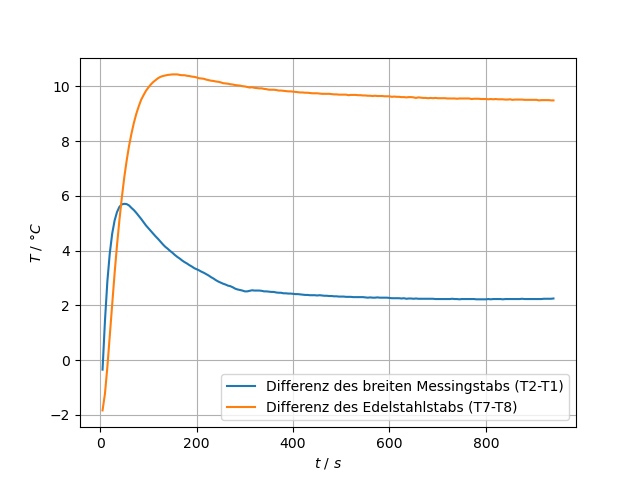
\includegraphics[height=80mm]{bilder/Tempdiff.png}
    \caption{Die Differenz der beiden Thermoelementen von dem breiten Messingstab und dem Edelstahlstab. \label{Abbildung5} }
\end{figure}

\begin{align*}
    \kappa_{\text{Aluminium}} = 237\,\frac{\unit{\watt}}{(\unit{\meter\kelvin})}\\
    \kappa_{\text{Edelstahl}} = 15\,\frac{\unit{\watt}}{(\unit{\meter\kelvin})}\\
    \kappa_{\text{Messing}} = 120\,\frac{\unit{\watt}}{(\unit{\meter\kelvin})}\\
    A_{\text{Messing(breit), Edelstahl(breit), Aluminium}} = 4,8 \cdot 10^{-5}\,\unit{\meter^2} \\
    A_{\text{Messing(schmal)}} = 2,8 \cdot 10^{-5}\,\unit{\meter^2}\\
    \increment x_{\text{Alle Stäbe}} = (0,035 \pm 0,000)\,\unit{\meter} 
\end{align*}

\begin{table}[H]
    \centering
    \caption{Der Wärmestrom pro Zeit der jeweiligen Temperaturdifferenz.}
    \label{Tabelle1}
    \begin{tabular} {c     c     c     c     c}
        \toprule
        {$ \text{Messzeit}\,\, t \mathbin{/} \unit{\second} $} &
        {$ T_{2} - T_{1} \mathbin{/} \unit{\kelvin}$} &
        {$ \frac{\increment Q_{\text{Messing(breit)}}}{\increment t}  \mathbin{/} \unit{\watt} $} &
        {$ T_{7} - T_{8}  \mathbin{/} \unit{\kelvin} $} &
        {$ \frac{\increment Q_{\text{Edelstahl}}}{\increment t}  \mathbin{/} \unit{\watt} $} \\
        \midrule
        100 & 4,7 & -0,7734 & 10,0 & -0,2057 \\
        200 & 3,3 & -0,5430 & 10,4 & -0,2139 \\
        400 & 2,4 & -0,3949 & 9,7  & -0,1968 \\
        600 & 2,3 & -0,3785 & 9,55 & -0,1964 \\
        800 & 2,2 & -0,3620 & 9,53 & -0,1960 \\
        \bottomrule
    \end{tabular} 
\end{table}

\begin{table}[H]
    \centering
    \caption{Der Wärmestrom pro Zeit der jeweiligen Temperaturdifferenz.}
    \label{Tabelle2}
    \begin{tabular} {c     c     c     c     c}
        \toprule
        {$ \text{Messzeit}\,\, t \mathbin{/} \unit{\second} $} &
        {$ T_{6} - T_{5} \mathbin{/} \unit{\kelvin}$} &
        {$ \frac{\increment Q_{\text{Aluminium}}}{\increment t}  \mathbin{/} \unit{\watt} $} &
        {$ T_{3} - T_{4}  \mathbin{/} \unit{\kelvin} $} &
        {$ \frac{\increment Q_{\text{Messing(schmal)}}}{\increment t}  \mathbin{/} \unit{\watt} $} \\
        \midrule
        100 & 3    & -0,9750 & 5,54 & -0,5318 \\
        200 & 1,90 & -0,6175 & 4,63 & -0,4444 \\
        400 & 1,54 & -0,5005 & 3,54 & -0,3398 \\
        600 & 1,50 & -0,4875 & 3,50 & -0,3360 \\
        800 & 1,48 & -0,4810 & 3,45 & -0,3312 \\
        \bottomrule
    \end{tabular} 
\end{table}

\begin{flushleft}
    Beide Graphen verhalten sich am Anfang ähnlich, sie nehmen beide stark zu. 
    Doch der Messingstab besitzt ungefähr bei $ 5\,\unit{\degreeCelsius} $ einen Hochpunkt. 
    Die Temperatur sinkt ab dem Punkt und bildet eine Asymptote bei ungefähr $ 2\,\unit{\degreeCelsius} $.
    Verglichen mit dem Edelstahlstab, nimmt der exponentiell zu um ungefähr $ 11\,\unit{\degreeCelsius} $ und bildet einen kleinen Hochpunkt. 
    Wie beim Messingstab, verhält sich der Edelstahlstab asymptotisch bei ungefähr $ 9,5\,\unit{\degreeCelsius} $ mit ausnehmender Zeit.
\end{flushleft}

\vspace{1cm}

\underline{\textbf{Dynamische Methode}}

\begin{flushleft}
    In diesem Teil werden die Temperaturverläufe periodisch dargestellt und daraus die Wärmeleitfähigkeit $\kappa$ bestimmt.
    Dazu werden die Elemente, Messing und Aluminium, bei einer Periode von jeweils $80\,\unit{\second}$ erhitzt und gekühlt.
    Die Amplituden, $A_{\text{Nah}}$ und $A_{\text{Fern}}$, sowie die Phasendifferenz $\increment t$, werden abgelesen, gemittelt und die dazugehörige Abweichung bestimmt.
    Die Wärmeleitfähigkeit wird mit der Formel \ref{6} bestimmt.
    Die Materialkonstanten werden entnommen aus, dem Arbeitblatt \cite{a1}.
\end{flushleft}


\begin{figure}[H]
    \centering
    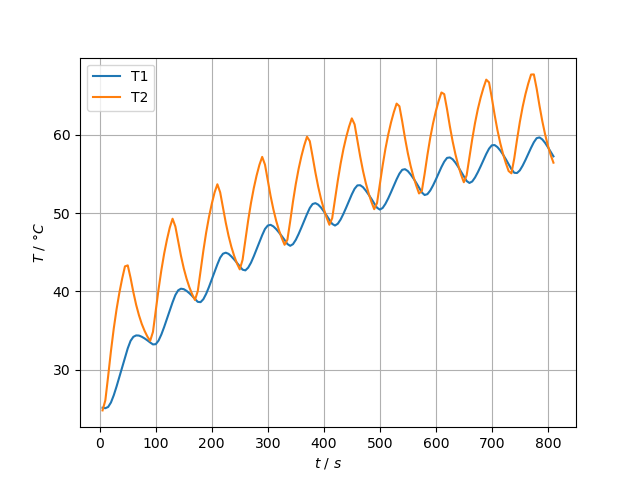
\includegraphics[height=80mm]{bilder/TemprVerlDyT1T2.png}
    \caption{Die Abbildung der zeitlichen Temperaturverläufe, mit der dynamischen Methode, der beiden Thermoelementen von dem breiten Messingstab.\label{Abbildung6} }
\end{figure}

\begin{align*}
    \rho_{\text{breiter Messing}} = 8520\,\frac{\unit{\kilo\gram}}{\unit{\meter^3}}\\
    c_{\text{breiter Messing}} = 385\, \frac{\unit{\joule}}{(\unit{\kilo\gram\kelvin})} \\
    \increment x = (0,035 \pm 0,000)\,\unit{\meter}\\
\end{align*}

\begin{table}[H]
    \centering
    \caption{Der Temperaturverlauf eines Messingstabes bei einer Periodendauer von $80\,\unit{\second}$.}
    \label{Tabelle2}
    \begin{tabular} {c     c     c     c     c}
        \toprule
        {$ A_{\text{Nah}}  \mathbin{/} \unit{\kelvin} $} &
        {$ A_{\text{Fern}} \mathbin{/} \unit{\kelvin}$} &
        {$ ln\left(\frac{A_{\text{Nah}}}{A_{\text{Fern}}}\right)$} &
        {$ \text{Phasendifferenz}\,\, \increment t  \mathbin{/} \unit{\second} $} \\
        \midrule
         7,69 & 3,84 & 0,69 & 12,20 \\
         8,07 & 3,07 & 0,96 & 16,65 \\
         7,30 & 3,03 & 0,87 & 12,20 \\
         6,90 & 2,96 & 0,84 & 12,20 \\
         6,88 & 2,46 & 1,02 & 11,65 \\
        10,0 & 3,17 & 1,14 & 27,75 \\
         6,92 & 2,69 & 0,94 & 16,70 \\
         6,73 & 2,30 & 1,07 & 12,21 \\
         7,30 & 2,34 & 1,13 & 10,99 \\
         7,50 & 2,26 & 1,19 &  8,88 \\
        \bottomrule
    \end{tabular} 
\end{table}

\begin{align*}
    A_{\text{Nah}} = (7,529 \pm 1,055)\,\unit{\kelvin}\\
    A_{\text{Fern}} = (2,812 \pm 0,499)\,\unit{\kelvin}\\
    \increment t = (14,143 \pm 1,053)\,\unit{\second}\\
    ln\left(\frac{A_{\text{Nah}}}{A_{\text{Fern}}}\right) = (0,985 \pm 0,156)\\
\end{align*}

\begin{align*}
    \intertext{Daraus folgt für $\kappa$ aus der Formel (\ref{6}) }\\
    \kappa = (144,221 \pm 2,962)\,\frac{\unit{\watt}}{(\unit{\meter\kelvin})}.\\
\end{align*}

\begin{figure}[H]
   \centering
    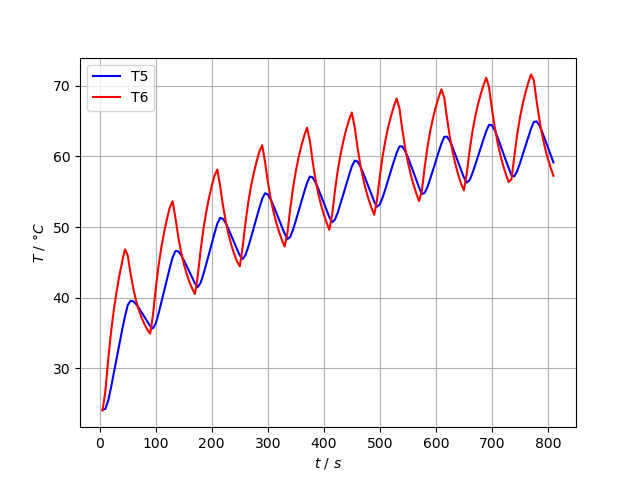
\includegraphics[height=80mm]{bilder/TemprVerlDyT5T6.png}
    \caption{Die Abbildung der zeitlichen Temperaturverläufe, mit der dynamischen Methode, der beiden Thermoelementen von dem Aluminiumstab.\label{Abbildung7} }
\end{figure}

\begin{align*}
    \rho_{\text{Aluminiumstab}} = 2800\,\frac{\unit{\kilo\gram}}{\unit{\meter^3}}\\
    c_{\text{Aluminiumstab}} = 830\, \frac{\unit{\joule}}{(\unit{\kilo\gram\kelvin})} \\
    \increment x = (0,035 \pm 0,000)\,\unit{\meter}\\
\end{align*}

\begin{table}[H]
    \centering
    \caption{Der Temperaturverlauf eines Aluminiumstabes bei einer Periodendauer von $80\,\unit{\second}$.}
    \label{Tabelle3}
    \begin{tabular} {c     c     c     c     c}
        \toprule
        {$ A_{\text{Nah}}  \mathbin{/} \unit{\kelvin} $} &
        {$ A_{\text{Fern}} \mathbin{/} \unit{\kelvin}$} &
        {$ ln\left(\frac{A_{\text{Nah}}}{A_{\text{Fern}}}\right)$} &
        {$ \text{Phasendifferenz}\,\, \increment t  \mathbin{/} \unit{\second} $} \\
        \midrule
        10,00 & 5,41 & 0,61 & 10,54 \\
         9,16 & 4,16 & 0,78 &  7,70 \\
         8,75 & 4,12 & 0,75 & 11,10 \\
         8,41 & 4,08 & 0,72 &  9,43 \\
         8,30 & 4,00 & 0,72 &  9,80 \\
        10,41 & 6,60 & 0,45 & 11,10 \\
         8,20 & 4,17 & 0,67 & 10,54 \\
         8,70 & 4,12 & 0,74 &  9,43 \\
         8,31 & 4,20 & 0,68 & 10,87 \\
         7,49 & 4,15 & 0,59 & 11,65 \\
        \bottomrule
    \end{tabular} 
\end{table}

\begin{align*}
    A_{\text{Nah}} = (8,772 \pm 0,874)\,\unit{\kelvin}\\
    A_{\text{Fern}} = (4,501 \pm 0,853)\,\unit{\kelvin}\\
    \increment t = (10,216 \pm 1,146)\,\unit{\second}\\
    ln\left(\frac{A_{\text{Nah}}}{A_{\text{Fern}}}\right) = (0,671 \pm 0,098)\\
\end{align*}

\begin{align*}
    \intertext{Daraus folgt für $\kappa$, mit der Formel (\ref{6}) }\\
    \kappa = (207,653 \pm 2,517)\,\frac{\unit{\watt}}{(\unit{\meter\kelvin})}.\\
\end{align*}

\begin{figure}[H]
    \centering
    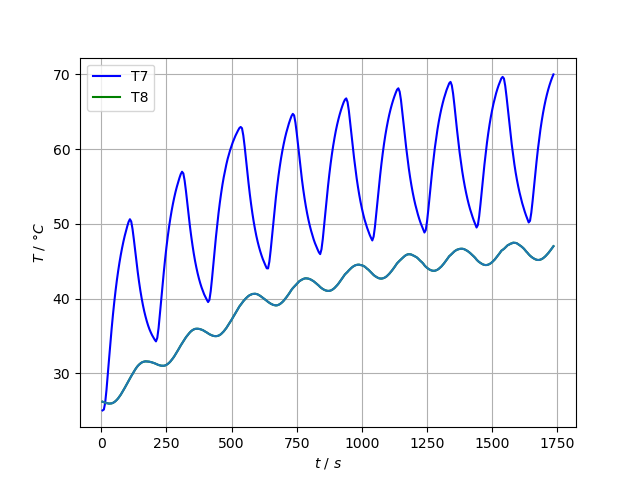
\includegraphics[height=80mm]{bilder/TemprVerlDyT7T8.png}
    \caption{Die Abbildung der zeitlichen Temperaturverläufe, mit der dynamischen Methode, der beiden Thermoelementen von dem Edelstahlstab.\label{Abbildung8} }
\end{figure}

\begin{align*}
    \rho_{\text{Edelstahlstab}} = 8000\,\frac{\unit{\kilo\gram}}{\unit{\meter^3}}\\
    c_{\text{Edelstahlstab}} = 385\, \frac{\unit{\joule}}{(\unit{\kilo\gram\kelvin})} \\
    \increment x = (0,035 \pm 0,000)\,\unit{\meter}\\
\end{align*}

\begin{table}[H]
    \centering
    \caption{Der Temperaturverlauf eines Edelstahlstabes bei einer Periodendauer von $200\,\unit{\second}$.}
    \label{Tabelle4}
    \begin{tabular} {c     c     c     c     c}
        \toprule
        {$ A_{\text{Nah}}  \mathbin{/} \unit{\kelvin} $} &
        {$ A_{\text{Fern}} \mathbin{/} \unit{\kelvin}$} &
        {$ ln\left(\frac{A_{\text{Nah}}}{A_{\text{Fern}}}\right)$} &
        {$ \text{Phasendifferenz}\,\, \increment t  \mathbin{/} \unit{\second} $} \\
        \midrule
        11,20 & 1,68 & 1,89 & 51,13 \\
        12,10 & 1,92 & 1,83 & 48,86 \\
        10,40 & 1,52 & 1,92 & 52,30 \\
        10,00 & 1,40 & 1,96 & 53,30 \\
        11,90 & 1,60 & 2,00 & 46,60 \\
        12,80 & 2,48 & 1,64 & 47,71 \\
        11,60 & 1,52 & 2,03 & 46,44 \\
        11,08 & 1,60 & 1,93 & 49,98 \\
        \bottomrule
    \end{tabular} 
\end{table}

\begin{align*}
    A_{\text{Nah}} = (11,385 \pm 1,06)\,\unit{\kelvin}\\
    A_{\text{Fern}} = (1,715 \pm 0,343)\,\unit{\kelvin}\\
    \increment t = (49,54 \pm 1,79)\,\unit{\second}\\
    ln\left(\frac{A_{\text{Nah}}}{A_{\text{Fern}}}\right) = (1,9 \pm 0,122)\\
\end{align*}


\begin{align*}
    \intertext{Daraus folgt nach der Formel (\ref{6})}\\
    \kappa = (20,19 \pm 0,748)\,\frac{\unit{\watt}}{(\unit{\meter\kelvin})}.\\
\end{align*}